\documentclass[preview]{standalone}
\usepackage{tikz}
\usepackage{circuitikz}
\usetikzlibrary{shapes.misc}
\usetikzlibrary{decorations.markings, arrows}

\begin{document}
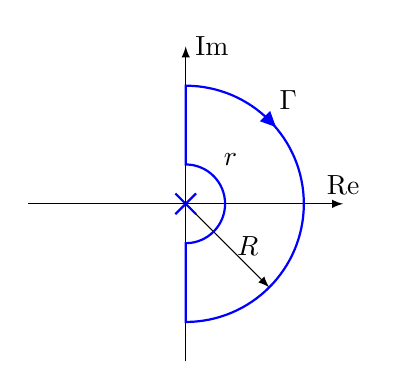
\begin{tikzpicture}
  \draw[-latex] (0,0) node[draw, blue, thick, cross out]{} -- node[right]{$R$} (-45:1.5) {};
  \draw[-latex] (-2,0) -- (2,0) node[above] {Re};
  \draw[-latex] (0,-2) -- (0,2) node[right] {Im};
  \draw[blue, thick] (0,1.5) arc (90:-90:1.5) node[color=blue, currarrow, sloped, pos=0.25]{} node[black, pos=0.25, above right]{$\Gamma$} -- (0,-0.5) arc (-90:90:0.5) node[black, pos=0.75, above right]{$r$} -- cycle;
\end{tikzpicture}
\end{document}
